\section{Analyse de marché}

\subsection{Win-posturo}

WIN-POSTURE NV Software est une plateforme d'analyse en posturographie statique. 
Elle se distingue par sa convivialité et son ergonomie, facilitant son utilisation. 
Il offre la possibilité de créer et de gérer des protocoles d'acquisition tout en permettant de paramétrer des normes conformes aux recommandations de l'AFP85 (SOFPEL). 
Ce logiciel intègre des fonctionnalités avancées telles que l'analyse fractale et l'analyse par ondelette. 
Il permet également de comparer les résultats des examens pour chaque patient, avec des données facilement exportables vers Excel. 
Les rapports et bilans générés sont entièrement personnalisables, et le logiciel propose des outils intégrés pour la création de courriers et le publipostage.

\begin{figure}[ht]
    \centering
    \begin{subfigure}[b]{0.45\textwidth}
      \centering
      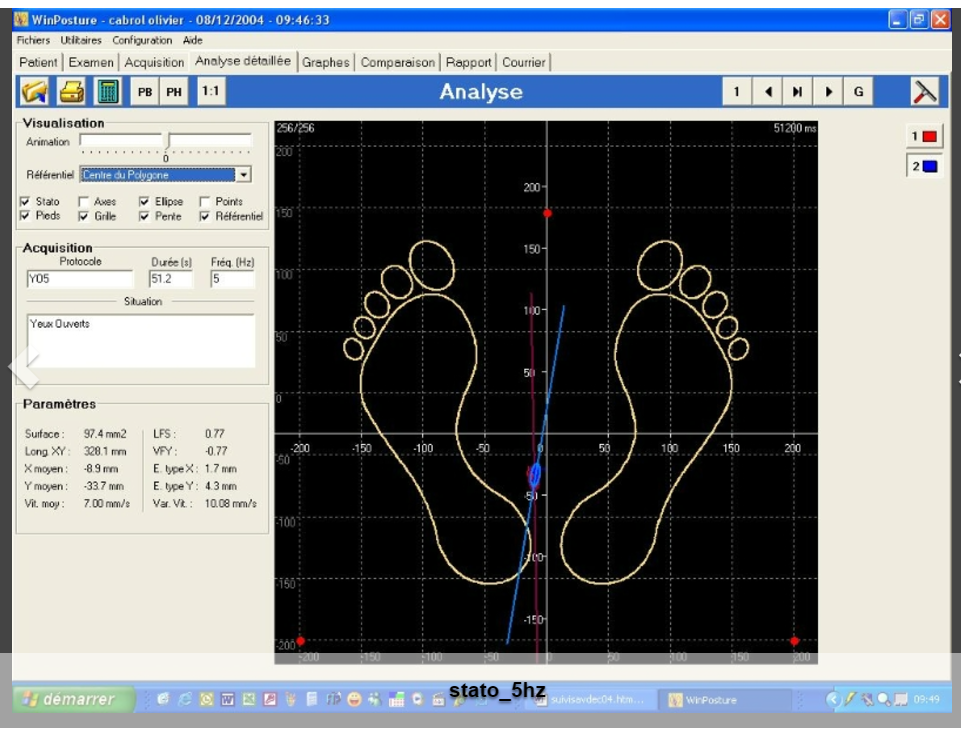
\includegraphics[height=5cm]{images/pression_plantaire/winposture.png}
      \caption{Logiciel Winposture}\label{fig:winposture}
    \end{subfigure}
    \begin{subfigure}[b]{0.5\textwidth}
        \centering
        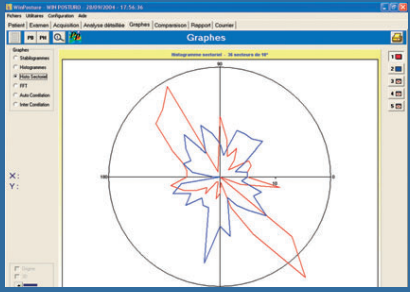
\includegraphics[height=5cm]{images/analyse_marche/winposture_ellipse.png}
        \caption{Visualisation de l'ellipse de confiance}\label{fig:winposture_ellipse_de_confiance}
    \end{subfigure}
    \begin{subfigure}[b]{0.5\textwidth}
        \centering
        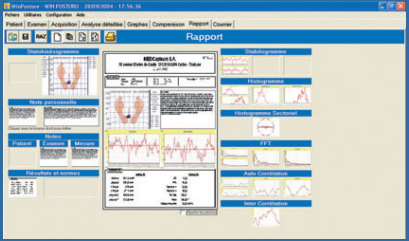
\includegraphics[height=5cm]{images/analyse_marche/winposture_rapport.png}
        \caption{Rapport du logiciel sur un cas patient}\label{fig:winposture_rapport}
    \end{subfigure}
    \begin{subfigure}[b]{0.5\textwidth}
        \centering
        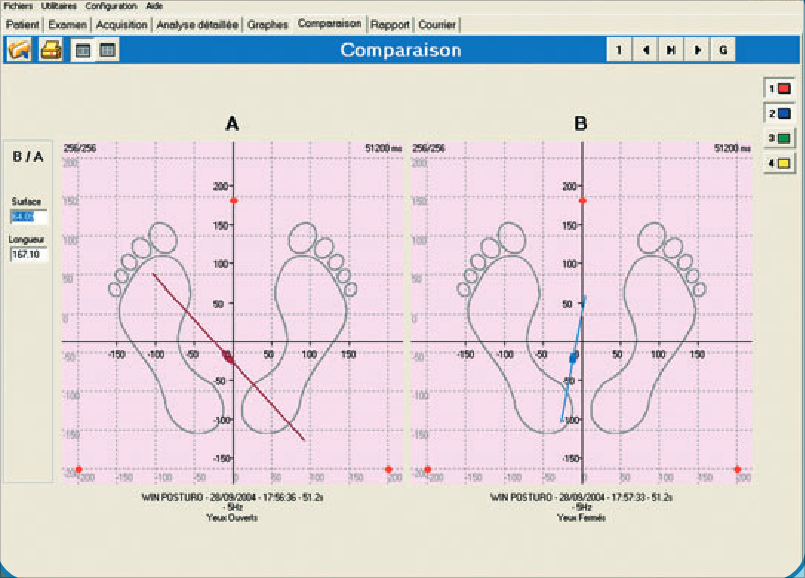
\includegraphics[height=5cm]{images/analyse_marche/comparaison_yo_yf.png}
        \caption{Comparaison de l'équilibre orthostatique yeux ouverts/fermés}\label{fig:winposture_comparaison_yo_yf}
    \end{subfigure}
\end{figure}

\subsection{Fusyo}

Fusyo combine analyses stabilométriques et baropodométriques pour une évaluation complète de \\ l'équilibre et des pressions plantaires. 
Cette plateforme d'analyse se distingue par ses visualisations avancées, notamment en thermographie, 3D et isopression. 
Il inclut des indicateurs tels que le Foot Posture Index, offrant une précision précieuse pour des analyses cliniques approfondies. 
Il permet de créer et gérer des protocoles d'acquisition tout en fournissant des données stabilométriques normalisées selon l'APE 85. 
Les résultats sont personnalisables et peuvent être facilement comparés entre les examens.

